\documentclass[aspectratio=169,11pt]{beamer}
\usepackage[T1]{fontenc}
\usepackage[utf8]{inputenc}
\usepackage{lmodern}
\usepackage{graphicx}
\usepackage{booktabs}
\usepackage{amsmath,amssymb}
\usepackage{xcolor}

\graphicspath{
    {../results/slide_figs/}
    {../results/report_figs/}
    {results/slide_figs/}
    {results/report_figs/}
}

\usetheme{default}
\usecolortheme{whale}
\setbeamertemplate{navigation symbols}{}
\setbeamertemplate{footline}[frame number]
\setbeamercolor{title}{fg=structure!80!black}
\setbeamerfont{frametitle}{size=\large,series=\bfseries}
\setbeamerfont{title}{size=\Large,series=\bfseries}
\setbeamertemplate{itemize item}{\color{structure}\textbullet}

% Show notes interleaved with slides
\setbeameroption{show notes}
\setbeamertemplate{note page}[plain]

\title{0--k BFS}
\subtitle{Bounded Integer Weights Shortest Path -- C++17}
\author{Artemov Makar \and Mark Shkut}
\institute{Skoltech, Algorithms 2026}
\date{May 21, 2026}

\begin{document}

% ------------------------------------------------------------- 1: TITLE
\begin{frame}
  \titlepage
\end{frame}
\note{
\textbf{Open with the headline.}\\[0.4em]
Project: 0--k BFS for the bounded-integer-weights shortest path problem in
C++17. Joint work with Mark. Goal of this presentation: explain the
algorithm family, show why it beats Dijkstra on graphs with small integer
weights, and present our measurements up to V = 9 $\cdot$ 10$^8$. Keep it tight:
about 15 minutes plus questions.
}

% ------------------------------------------------------------- 2: PROBLEM
\begin{frame}{The problem}
\begin{itemize}
  \item Single-source shortest path on $G=(V,E,w)$
  \item Weights restricted to $\{0,1,\dots,k\}$ for small known $k$
  \item Target: $V$ approaching $10^9$ on a single workstation
\end{itemize}
\vspace{0.6em}
\textbf{Where this comes up:} grid path planning, layered graphs, 2-SAT-style
reductions, transport networks with a few toll levels.
\end{frame}
\note{
\textbf{Define the problem precisely.}\\
We want all distances from one source. The catch is that the weights are
non-negative integers bounded by a small $k$. This restriction is not
artificial: it shows up constantly in pathfinding on grids, in layered
DAGs, and in competitive programming. The reason it is interesting from
an algorithms standpoint is that we can do better than the classical
$O((V+E)\log V)$ Dijkstra by exploiting the small range of weights.\\
\textbf{Why the V $\to 10^9$ target:} we set this as a forcing function
on the design -- it dictates the implicit-graph backend and the 32-bit
distance type that come later.
}

% ------------------------------------------------------------- 3: BASELINE
\begin{frame}{Baseline: Dijkstra}
\begin{itemize}
  \item \texttt{std::priority\_queue<pair<Distance,Vertex>>}, lazy decrease-key
  \item $O((V+E)\log V)$ time, $O(V+E)$ memory
  \item Works for any non-negative real weights
\end{itemize}
\vspace{0.4em}
The $\log V$ factor is the cost of the priority queue. \emph{If we know
weights are bounded, can we replace it with something cheaper?}
\end{frame}
\note{
\textbf{Set up Dijkstra as the benchmark to beat.}\\
This is the standard algorithm everyone knows. We implement it
straightforwardly: a heap of (distance, vertex) pairs with lazy
decrease-key (re-push, skip stale on pop). The $\log V$ factor sits
inside every relaxation that improves a distance. The whole point of
0--k BFS is that when the weights are small integers, you do not need a
heap at all.\\[0.3em]
\textit{Pause for the question on the slide -- this motivates the next
slide.}
}

% ------------------------------------------------------------- 4: 0-1 BFS
\begin{frame}{The trick: 0--1 BFS}
Weights are 0 or 1. Replace the priority queue with a \textbf{deque}:
\begin{itemize}
  \item edge of weight 0 $\to$ \texttt{push\_front}
  \item edge of weight 1 $\to$ \texttt{push\_back}
\end{itemize}
\vspace{0.3em}
The deque is always sorted by distance, in two contiguous layers.
\begin{center}
\textbf{Complexity:}\quad $O(V+E)$\qquad
\textbf{Memory:}\quad $O(V)$
\end{center}
\end{frame}
\note{
\textbf{Pedagogical core, part 1.}\\
The idea is simple. Inside any BFS we always have ``current layer'' and
``next layer''. With 0/1 weights, a 0-edge keeps us in the current layer
(front of the deque, processed immediately) and a 1-edge moves us to
the next layer (back of the deque). The deque stays sorted by distance
with at most two distinct values at any time.\\
Important detail vs.\ plain BFS: a vertex can be discovered multiple
times before it is final, so we must check
\emph{dist[v] + w(v,u) < dist[u]} on every relaxation, not just
``visited or not''.
}

% ------------------------------------------------------------- 5: 0-k BFS
\begin{frame}{Generalize: 0--k BFS}
Weights are $\{0,1,\dots,k\}$. Use \textbf{$k+1$ FIFO queues}, indexed by
$\mathrm{dist}[v] \bmod (k+1)$.
\begin{itemize}
  \item ``Active'' bucket $\mathrm{cur}$ walks forward
  \item Relaxation pushes $v$ into bucket $(d_{\text{new}}) \bmod (k+1)$
  \item Stale entries are skipped on pop
\end{itemize}
\begin{center}
\textbf{Complexity:}\quad $O(kV+E)$\qquad
\textbf{Memory:}\quad $O(k+E)$ for queues
\end{center}
\end{frame}
\note{
\textbf{Pedagogical core, part 2.}\\
Generalize: with weights up to $k$, a vertex relaxed at distance $d$
moves at most $d+k$ steps forward. So at any moment, only $k+1$
``layers'' of distance values are alive. We allocate $k+1$ FIFO queues
and index them by $\text{dist} \bmod (k+1)$ -- a circular buffer of
buckets.\\
This is why it is called ``circular FIFO queues''. The \texttt{cur}
pointer walks through them; when the current bucket empties, we
advance to the next. If a vertex is re-relaxed to a smaller distance,
it lands in a different bucket, and the original slot becomes a stale
entry that we skip on pop.
}

% ------------------------------------------------------------- 6: VISUAL
\begin{frame}{What it looks like}
\centering
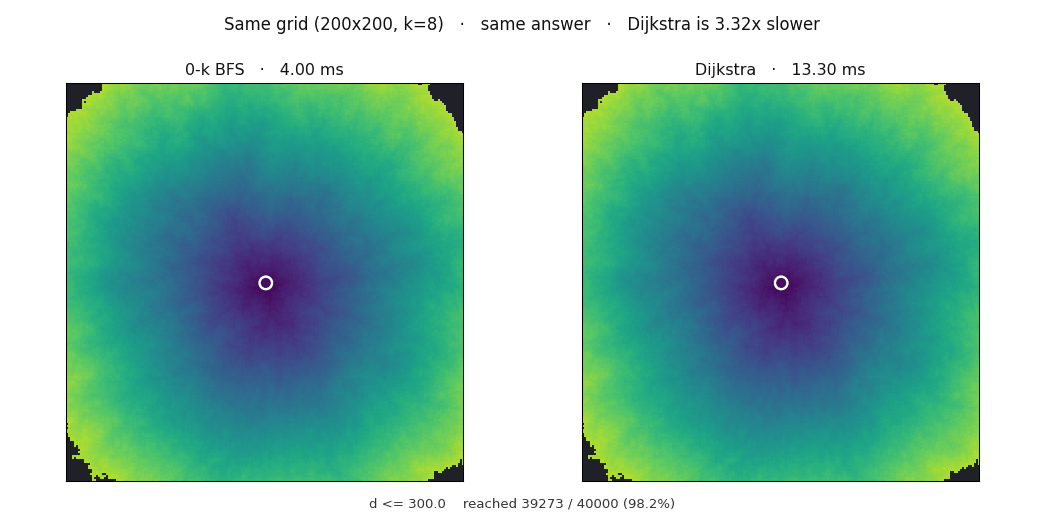
\includegraphics[width=0.86\linewidth]{compare_still.png}
\\[0.2em]
\footnotesize Same 200$\times$200 grid, $k=8$. Same answer.
0--k BFS \textbf{4.00 ms}, Dijkstra \textbf{13.30 ms} -- 3.32$\times$ slower.
\end{frame}
\note{
\textbf{Show the comparison animation (or this still).}\\
``Both algorithms produce the same distance field. The left panel finishes
the wavefront in 4 milliseconds, the right one in 13.3 milliseconds
because every relaxation pays the log-factor in the heap. The animation
in the repository runs this live -- you can see both wavefronts filling
in lockstep with the real times in the titles.''\\
\textbf{Talking point:} the visualization is also part of the project --
it is how we communicated the work to ourselves before benchmarking.
}

% ------------------------------------------------------------- 7: QUEUES
\begin{frame}{Under the hood}
\centering
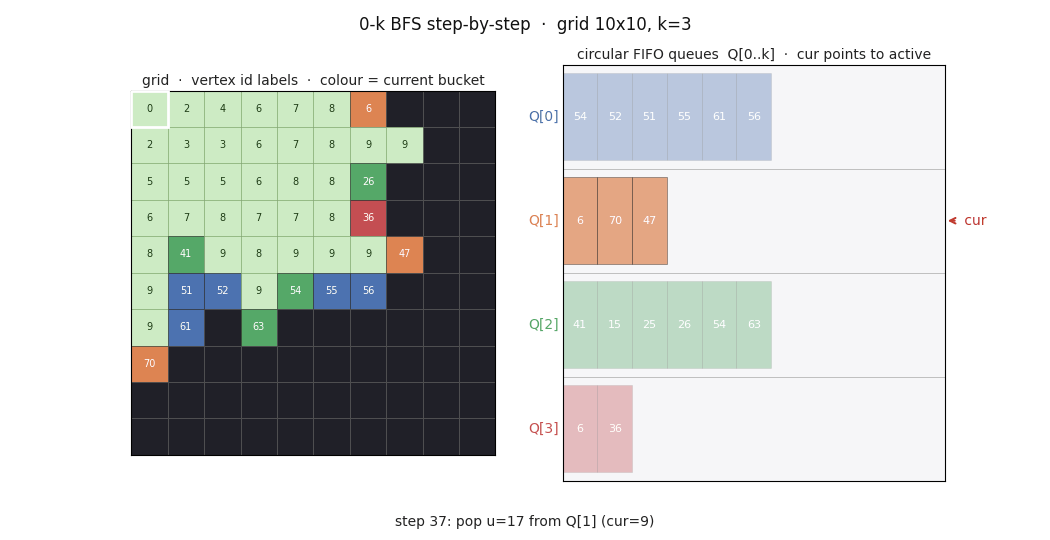
\includegraphics[width=0.85\linewidth]{queues_still.png}
\\[0.2em]
\footnotesize Step-by-step on a tiny $10\times10$ grid, $k=3$.\,
Each row on the right is one queue $Q[0]\dots Q[3]$; \,
\textcolor{red}{\textbf{cur}} marks the active bucket.
\end{frame}
\note{
\textbf{Anchor the data structure.}\\
On the right you see the actual four queues $Q[0]$ through $Q[3]$ with
their current contents (the numbers are vertex ids). On the left you see
the grid, with cells coloured by which bucket currently owns them. The
\texttt{cur} pointer is on $Q[1]$ in this frame.\\
The animation is in \texttt{viz/animate\_queues.py} and it consumes a
per-step trace dumped by the instrumented C++ algorithm
(\texttt{include/zkbfs/bfs0k\_trace.hpp}). This is the part that makes
the algorithm \emph{teachable} -- the queues are the whole secret.
}

% ------------------------------------------------------------- 8: SCALE
\begin{frame}{Designing for V $\to 10^9$}
\begin{itemize}
  \item Explicit CSR at $V=10^9$ costs $\sim$20 GB just for edges -- \emph{infeasible}
  \item \texttt{GridGraph}: implicit 4-neighbour grid, $O(1)$ neighbour function, no edge storage
  \item \texttt{Distance = uint32\_t}: halves the dominant array (4 GB instead of 8 GB)
  \item Trade-off only valid while $k \cdot V < 2^{32}$
\end{itemize}
\end{frame}
\note{
\textbf{Defend the design decisions that made the big run possible.}\\
We split the project into two backends. The general \texttt{GraphCSR}
caps out around $V \approx 10^8$ because of memory. The
\texttt{GridGraph} is implicit -- we do not store edges at all, we
compute them on the fly. That, plus a 32-bit distance type, is what
let us actually run on $V = 9 \cdot 10^8$ within 14 GB of free RAM.\\
Honest disclaimer: the 32-bit distance is not always safe. We require
$k \cdot V < 2^{32}$. For the parameters we care about, this is fine,
and we have a 64-bit fallback via a compile flag.
}

% ------------------------------------------------------------- 9: RESULTS
\begin{frame}{Results, grid, single thread}
\centering
\small
\begin{tabular}{rrrrr@{}r}
\toprule
$V$            & $k$ & Dijkstra & 0--k BFS & 0--1 BFS & speed-up \\ \midrule
$10^6$         & 1   & 0.180 s  & 0.039 s  & 0.070 s  & 4.6$\times$ \\
$10^7$         & 1   & 1.98 s   & 0.493 s  & 0.355 s  & 5.6$\times$ \\
$10^8$         & 1   & 60.3 s   & 28.4 s   & 5.44 s   & \textbf{11.1}$\times$ \\
$4.84\cdot 10^8$ & 4 & 432.9 s  & 451.4 s  & ---      & 0.96$\times$ (mem) \\
\textbf{$9\cdot 10^8$} & 1 & \textbf{619.9 s} & --- & \textbf{121.2 s} & \textbf{5.12}$\times$ \\
\bottomrule
\end{tabular}
\\[0.6em]
Both algorithms produce \emph{byte-identical} distance checksums on every
graph instance.
\end{frame}
\note{
\textbf{Walk the table top to bottom.}\\
At $V=10^6$ we already get a 4--5$\times$ speed-up. At $V=10^8$ with
$k=1$, the deque-based 0--1 BFS is 11$\times$ faster than Dijkstra. The
$V \approx 5 \cdot 10^8$ row is interesting -- the gap collapses
because both algorithms become memory-bandwidth bound. The bottom row
is the headline: on 900 million vertices, 0--1 BFS finishes in two
minutes, Dijkstra takes ten.\\
Critically, all checksums match -- correctness was verified across 19
distinct graph instances in the sweep, zero mismatches.
}

% ------------------------------------------------------------- 10: PLOT
\begin{frame}{Scaling}
\centering
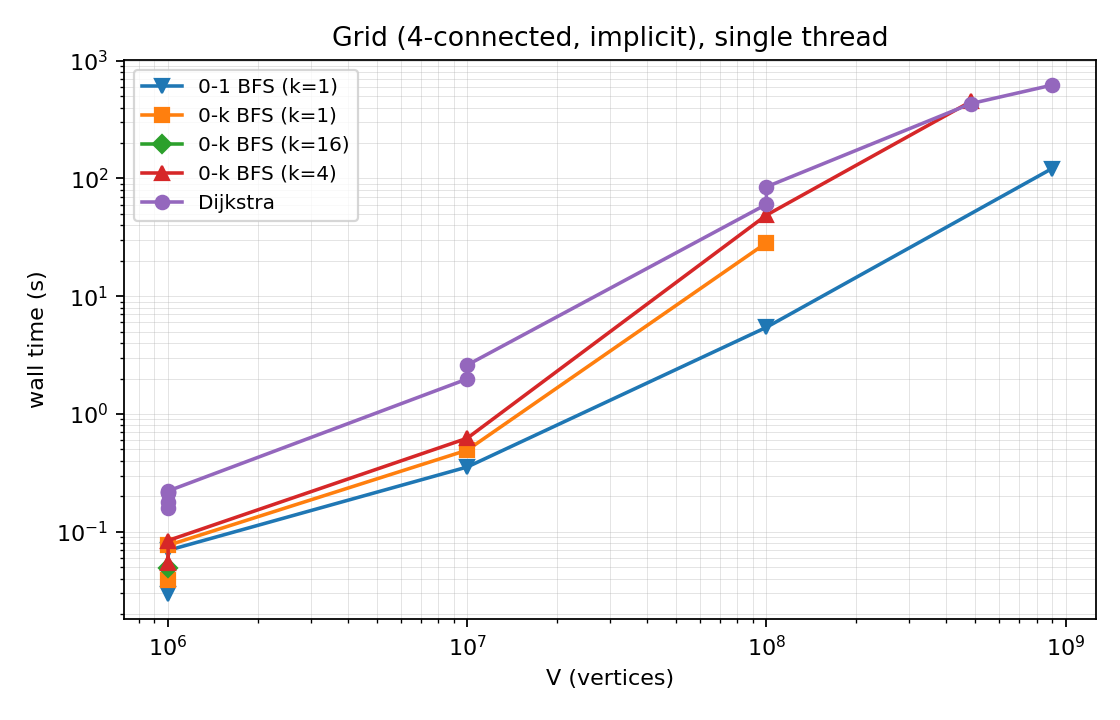
\includegraphics[width=0.72\linewidth]{grid_scaling.png}
\end{frame}
\note{
\textbf{Walk the plot.}\\
Both axes are log scale. Five series: Dijkstra at the top, the BFS
variants tracking parallel below it. The constant vertical gap on the
log scale corresponds to a roughly constant multiplicative speed-up.
At $V=10^8$ and beyond, the lines start to converge as we move into the
memory-bound regime. The lowest line throughout is the deque-based 0--1
BFS, which is the cleanest implementation in the family.
}

% ------------------------------------------------------------- 11: LIMITS
\begin{frame}{Limits}
\begin{itemize}
  \item Speed-up shrinks as $k$ grows -- gone at $k = \omega(\log V)$
  \item At $V \gtrsim 5 \cdot 10^8$ both algorithms become memory-bandwidth bound
  \item Two-queue $bfs\_0k$ is slower than single-deque $bfs\_01$ at large $V$ (allocator overhead) -- $k+1$ queues = $k+1$ allocators
  \item Needs non-negative integer weights with known small $k$
\end{itemize}
\end{frame}
\note{
\textbf{Be honest about where this fails.}\\
First: this is a constant-factor win, not an asymptotic one. Once $k$ is
proportional to $\log V$, Dijkstra is at least as good.\\
Second: at huge $V$ everything is memory-bound. We measured the
0--k BFS slowing down to parity with Dijkstra at $V \approx 5 \cdot
10^8$. Implementation matters a lot: maintaining $k+1$ separate queue
allocators hurts cache and allocator pressure compared to one deque,
which is why our 0--1 BFS keeps winning at $V = 9 \cdot 10^8$ but the
generic 0--k BFS would not.\\
Third: this is not a replacement for Dijkstra in general. Real-valued
weights or unknown weight bounds -- use Dijkstra.
}

% ------------------------------------------------------------- 12: NEXT
\begin{frame}{Next steps}
\begin{itemize}
  \item Indexed $d$-ary heap Dijkstra (proper decrease-key)
  \item Chunked ring-buffer FIFO for \texttt{bfs\_0k} (close the gap to 0--1 BFS)
  \item Real road-network loader (DIMACS USA, weights quantised to $k=8$)
  \item Stretch: $\Delta$-stepping for parallel context
\end{itemize}
\end{frame}
\note{
\textbf{Forward look.}\\
Four items. The first two are implementation polish -- a real
decrease-key heap to be a fairer baseline, and a chunked queue to match
the deque's cache behaviour. Three: leave the synthetic-graph comfort
zone and try a real road network. Four: $\Delta$-stepping is the
canonical parallel relative of 0--k BFS; it would be nice to have for
context even if we do not push the parallel side hard.
}

% ------------------------------------------------------------- 13: END
\begin{frame}{Thank you}
\begin{itemize}
  \item Code, report, plots: \texttt{github.com/artemovmak/EffectiveAlgorithms}
  \item Stage~1 report: \texttt{stage1\_report.pdf}
\end{itemize}
\vspace{0.6em}
Questions?
\end{frame}
\note{
\textbf{Close.}\\
Everything -- the code, the LaTeX report, the animations,
reproducible build scripts -- lives in the GitHub repo. Hand off to
questions. Likely questions: \\[0.2em]
\textit{Q:} ``Why is 0--1 BFS faster than 0--k BFS at $k=1$?'' --
allocator overhead of two \texttt{std::queue}s vs a single
\texttt{std::deque}.\\
\textit{Q:} ``How did you verify correctness on a billion-vertex run?''
-- distance-sum checksums match Dijkstra exactly; no per-vertex
comparison needed because the sum already pins down the array.\\
\textit{Q:} ``What about parallelism?'' -- single thread throughout
Stage~1; $\Delta$-stepping is the planned Week~2 stretch goal.
}

\end{document}
